\documentclass[11pt,a4paper]{article}
\usepackage{geometry}
\geometry{a4paper,left=25mm,right=25mm}
\usepackage[utf8]{inputenc}
\usepackage[german]{babel}
\usepackage{amsmath}
\usepackage{amsfonts}
\usepackage{amssymb}
\usepackage{scrpage2}\pagestyle{scrheadings}
\usepackage[pdftex]{graphicx}
\ihead{Thomas Verweyen (759743) \\ Norman Vetter (749229)}
\setheadsepline{0.2pt}
\begin{document}
\begin{center}
\section*{ Theoretische Informatik 1 \\ Übung Blatt 7}
\end{center}
\ \\ \ \\
\subsection*{Aufgabe 7.1}
\paragraph*{a)}\ \\
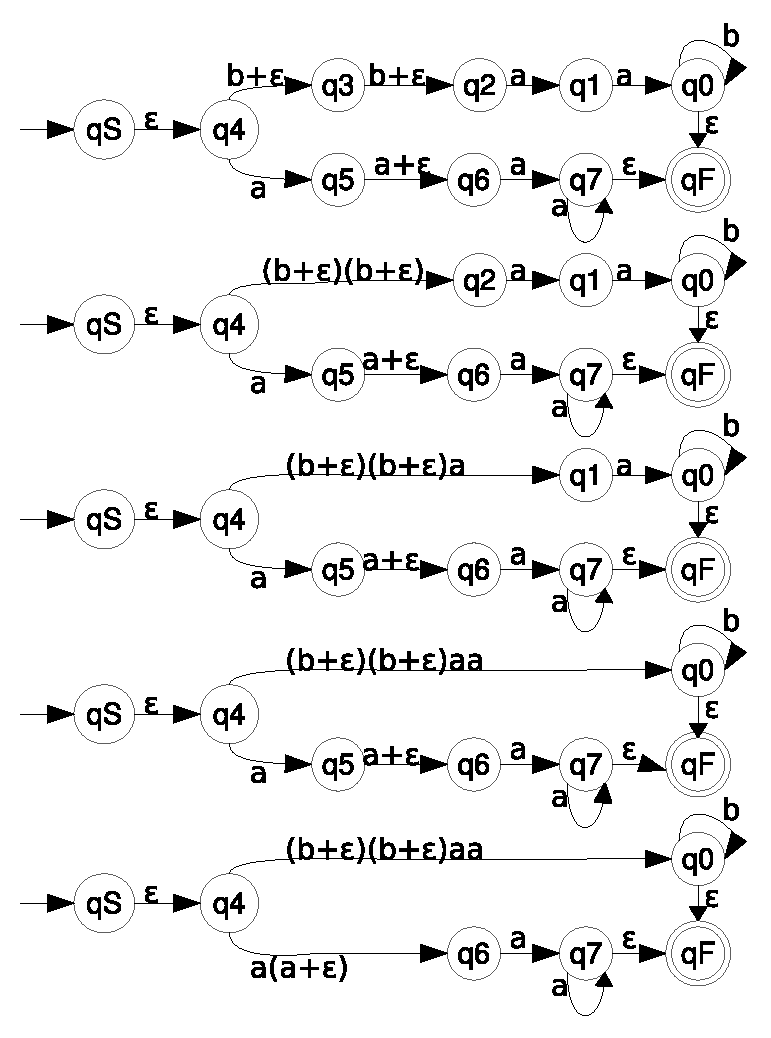
\includegraphics[scale=0.9]{71a.eps}\\
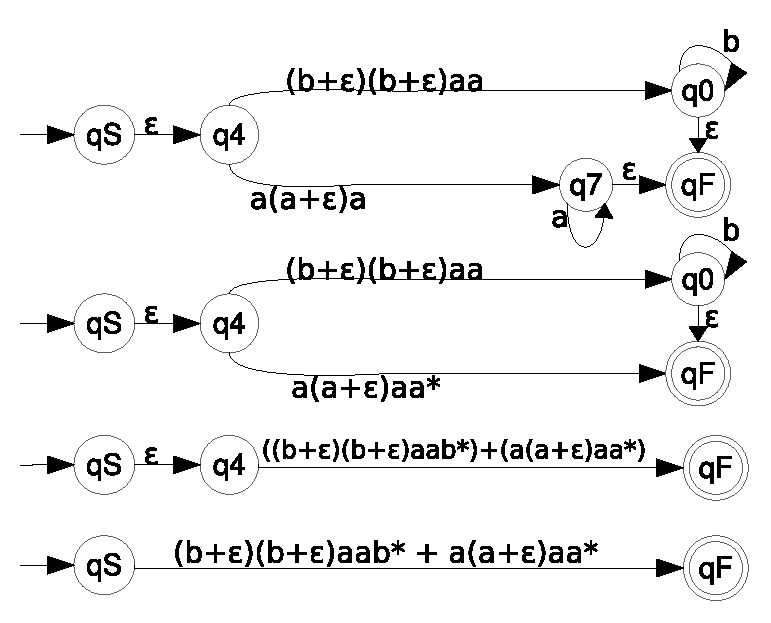
\includegraphics[scale=1]{71b.eps}\\
RA = (b+$\epsilon$)(b+$\epsilon$)aa$b^*$ + a(a+$\epsilon$)a$a^*$
\paragraph*{b)}\ \\
G=(\{S,A,B,C,D\},\{a,b\},P,S)\\
P:=\{$S \rightarrow AAaaC,S \rightarrow aBaD,A \rightarrow b,A \rightarrow \epsilon,B \rightarrow a, B \rightarrow \epsilon, C \rightarrow Cb,\\C \rightarrow \epsilon, D \rightarrow Da, D \rightarrow \epsilon$\}
\subsection*{Aufgabe 7.2}
\paragraph*{a)}\ \\
G=(\{S,T,U,V\}\{0,1,2\},P,S)\\
P:=\{$\overset{1}{\overbrace{S \rightarrow T}},\overset{2}{\overbrace{S \rightarrow 0T}},\overset{3}{\overbrace{S \rightarrow 0T0}},\overset{4}{\overbrace{S \rightarrow T0}},\overset{5}{\overbrace{T \rightarrow \epsilon}},\overset{6}{\overbrace{T \rightarrow 1T}},\overset{7}{\overbrace{T \rightarrow 2U}},\overset{8}{\overbrace{U \rightarrow 2V}},\overset{9}{\overbrace{V \rightarrow 2T}}$\}\\
w=0111222110\\
\ \\
Abarbeitung:\\
$S \overset{3}{\rightarrow} 0 \underline{T}0 \overset{6}{\rightarrow} 01 \underline{T}0 \overset{6}{\rightarrow} 011 \underline{T}0 \overset{6}{\rightarrow} 0111 \underline{T}0 \overset{7}{\rightarrow} 01112 \underline{U}0 \overset{8}{\rightarrow} 011122 \underline{V}0 \overset{9}{\rightarrow} 0111222 \underline{T}0 \overset{6}{\rightarrow} 01112221 \underline{T}0 \overset{6}{\rightarrow} 011122211 \underline{T}0 \overset{5}{\rightarrow} 0111222110$
\newpage
\paragraph*{b)}\ \\
L(G) = $(0+\epsilon)(1+222)^*(0+\epsilon)$\\
L ist allgemeingültig, expansiv, kontextfrei und linear aufgrund der Definitionen.\\
\begin{tabular}{ll}
Jedoch nicht
&kontextsensitiv da, $T \rightarrow \epsilon$\\
&rechtslinear da, $S \rightarrow T0$\\
&linkslinear da, $S \rightarrow 0T$\\
\end{tabular}
\paragraph*{c)}\ \\
G=(\{S,B,T,U,D\}\{0,1,2\},P,S)\\
P:=\{\\
% Bis hier Text ohne Einrückung
\begingroup
\leftskip=21mm
\noindent
% ab hier wieder Text ohne Einrückung
$S \rightarrow \epsilon|0B|1B|2T$,\\
$B \rightarrow \epsilon|1B|2T|0D$,\\
$T \rightarrow 2U$,\\
$U \rightarrow 2B$,\\
$D \rightarrow \epsilon$\}\\
\endgroup
RA = $(0+ \epsilon)(1+222)^*(0+ \epsilon )$
\subsection*{Aufgabe 7.3}
$G_k = (\{V_i| \forall i\in \mathbb{N}.1 \leq i \leq k \} , \{0\}, \{V_i \rightarrow 0V_{i+1}|\forall i\in \mathbb{N}.1\leq i < k\} \cup \{V_k \rightarrow \epsilon\}, V_1)$\\
L($G_k$) = $\{\underset{(k-1)mal}{\underbrace{0...0}}\}$\\
(1) Unsere Definition der Rechtslinearität erlaubt ausschließlich Regeln der Form:\\
$A \rightarrow \epsilon, A \rightarrow aB ~~~~~ (A,B \in V;a \in T)$\\
(2) In einer rechtslinearen Grammatik kann die Ableitung nie mehr als ein Nichtterminal enthalten (Definition).
(3) Damit keine unendliche Menge von Worten erzeugt wird, müssen Schleifen in den Produktionen vermieden werden, das heißt\\
$A \rightarrow^* wA~~~~~~~~~(A \in V, w \in T^*)$\\
darf nicht gelten.\\
Aufgrund der Regeln (1),(2) und (3) ist die einzige Möglichkeit das erzeugte Wort zu verlängern, Regeln der Form\\ 
$A \rightarrow aB~~~~~~~(A,B \in V, a \in T)$\\
zu verwenden.\\
Daraus folgt, dass um die Sprache über ein Wort w zu beschreiben, eine Nichtterminalmenge V benötigt wird, mit $|V| = |w| + 1$.

\end{document}